%
% 33-brachistochrone.tex
%
% (c) 2023 Prof Dr Andreas Müller
%

%
% Lösung des Brachistochronenproblems
%
\subsection{Lösung des Brachistochronenproblems
\label{buch:variation:eulerlagrange:subsection:brachistochrone}}
Das Brachistochronenproblem kann jetzt mit Hilfe der
Euler-Lagrange-Differentialgleichung gelöst werden.
Dazu muss zunächst die Lagrange-Funktion ermittelt werden,
mit der dann die Euler-Lagrange-Differentialgleichung aufgestellt
werden kann.
Dies erfordert einiges an Rechnung.
Schliesslich muss die Differentialgleichung gelöst werden.

%
% Lagrange-Funktion
%
\subsubsection{Lagrange-Funktion}
Die Lagrange-Funktion für das Brachistochronenproblem ist
\[
L(x,y,y')
=
\sqrt{\frac{1+y^{\prime 2}}{y}}.
\]
Diese Form des Variationsprinzips unterscheidet sich von der früher
gefundenen nur durch einen konstanten Faktor, der keinen Einfluss
auf die Lösung hat.

%
% Partielle Ableitungen der Lagrange-Funktion
%
\subsubsection{Partielle Ableitungen der Lagrange-Funktion}
Für die Euler-Lagrange-Differentialgleichung werden die partiellen
Ableitungen nach $y$ und $y'$ benöigt, sie sind
\begin{align*}
\frac{\partial L}{\partial y}
&=
-
\frac{\!\sqrt{1+y^{\prime 2}}}{2y^{\frac32}}
&&\Rightarrow
&\frac{\partial L}{\partial y}(x,y(x),y'(x))
&=
\frac{\!\sqrt{1+y'(x)^2}}{2y(x)^{\frac32}}
\\
\frac{\partial L}{\partial y'}
&=
\frac{y'}{\!\sqrt{y\cdot (1+y^{\prime 2})}}
&&\Rightarrow
&
\frac{\partial L}{\partial y'}(x,y(x),y'(x))
&=
\frac{y'(x)}{\!\sqrt{y(x)(1+y'(x)^2)}},
\end{align*}
wobei wir auf der rechten Seite bereits die Funktionen $y(x)$ und $y'(x)$
eingesetzt haben.
Für die Euler-Lagrange-Differentialgleichung muss die $y'$-Ableitung
nach $x$ ableiten werden, dies ergibt
\begin{align*}
\frac{d}{dx}
\frac{\partial L}{\partial y'}(x,y(x),y'(x))
&=
\frac{d}{dx}
\frac{y'(x)}{\!\sqrt{y(x)(1+y'(x)^2)}},
\\
&=
\frac{
y''(x)
\!\sqrt{y(x)(1+y'(x)^2)}
-
y'(x)
\displaystyle\frac{
		y'(x) (1+y'(x)^2) + 2y(x)y'(x)y''(x)
	}{
		2\sqrt{y(x)(1+y'(x)^2)}
}
}{
y(x)(1+y'(x)^2)
}
\\
&=
\frac{
2y''(x)
y(x)(1+y'(x)^2)
-
y'(x)
\bigl(y'(x)(1+y'(x)^2)+2y(x)y'(x)y''(x)\bigr)
}{
2\bigl(y(x)(1+y'(x)^2)\bigr)^{\frac32}
}
\\
&=
\frac{
2y(x)y''(x) + 2y(x)y'(x)^2y''(x)
-y'(x)^2-y'(x)^4-2y(x)y'(x)^2y''(x)
}{
2\bigl(y(x)(1+y'(x)^2)\bigr)^{\frac32}
}
\\
&=
\frac{
2y(x)y''(x) -y'(x)^2-y'(x)^4
}{
2\bigl(y(x)(1+y'(x)^2)\bigr)^{\frac32}
}
\intertext{Um den anderen Term der Euler-Lagrange-Differentialgleichung
auf den gleichen Nenner zu bringen, muss mit $(1+y'(x)^2)^\frac32$
erweitert werden:
}
\frac{\partial L}{\partial y}(x,y(x),y'(x))
&=
-
\frac{
(1+y'(x)^2)^2
}{
2\bigl(y(x)(1+y'(x)^2)\bigr)^{\frac32}
}
=
\frac{-1-2y'(x)^2-y'(x)^4}{
2\bigl(y(x)(1+y'(x)^2)\bigr)^{\frac32}
}
.
\end{align*}

%
% Euler-Lagrange-Differentialgleichung des Brachistochronenproblems
%
\subsubsection{Euler-Lagrange-Differentialgleichung des
Brachistochronenproblems}
Damit kann man jetzt die Euler-Lagrange-Differentialgleichung
\begin{align*}
0
&=
\frac{\partial L}{\partial y}(x,y(x),y'(x))
-
\frac{d}{dx}
\frac{\partial L}{\partial y'}(x,y(x),y'(x))
\\
&=
\frac{
-1 - 2y'(x)^2 - y'(x)^4
-2y(x)y''(x)+y'(x)^2+y'(x)^4
}{
2
\bigl(
y(x)
(1+y'(x)^2)
\bigr)^{\frac32}
}
\\
&=
\frac{
-1 - y'(x)^2
-2y(x)y''(x)
}{
2
\bigl(
y(x)
(1+y'(x)^2)
\bigr)^{\frac32}
}
\end{align*}
zusammenstellen.
\begin{equation}
1+y'(x)^2+2y(x)y''(x)=0
\qquad\Rightarrow\qquad
y''(x)
=
-\frac{1+y'(x)^2}{2y(x)}
\label{buch:variation:eulerlagrange:eqn:brachistochrone0}
\end{equation}
Diese Differentialgleichung ist nicht ganz einfach zu lösen.

%
% Reduktion auf eine Differentialgleichung erster Ordnung
%
\subsubsection{Reduktion auf eine Differentialgleichung erster Ordnung}
Der folgende Trick hilft mit der Lösung der Differentialgleichung weiter.
Wir mutliplizieren die Gleichung
\eqref{buch:variation:eulerlagrange:eqn:brachistochrone0}
mit $y'(x)$ und erhalten
\begin{equation}
y'(x) + 2y(x)y'(x)y''(x) + y'(x)^3 = 0.
\label{buch:variation:eulerlagrange:eqn:multiplikation}
\end{equation}
Die ist die Ableitung
\begin{align*}
\bigl(
y(x)(1+y'(x)^2)
\bigr)'
&=
y'(x)(1+y'(x)^2)
+
y(x)(2y'(x)y''(x))
\\
&=
y'(x) + y'(x)^3
+2y(x)y'(x)y''(x).
\end{align*}
Die ursprüngliche Differentialgleichung wird damit zur Gleichung
\[
\bigl(
y(x)(1+y'(x)^2)
\bigr)'
=
0,
\]
die integriert werden kann und
\[
y(x)(1+y'(x)^2)
=
C
\]
für eine Integrationskonstante $C$, die aus den Randbedingungen
ermittelt werden muss, ergibt.
Diese Differentialgleichung kann in die explizite Form
\begin{equation}
y'(x)
=
\sqrt{
\frac{C-y(x)}{y(x)}
}
\label{buch:variation:eulerlagrange:eqn:brachistochrone1}
\end{equation}
gebracht werden.
Dies ist die gesuchte Differentialgleichung erster Ordnung.

%
% Lösung in Parameterdarstellung
%
\subsubsection{Lösung in Parameterdarstellung}
Aus der optischen Analogie von Bernoulli wissen wir, dass die Lösungskurve
möglicherweise besser durch den Winkel zwischen der Kurve und der Vertikalen
parametrisiert werden kann.
Wir bezeichnen den Winkel mit $\vartheta$ und schreiben die Ableitung
\[
\frac{dy}{dx}
=
\cot \vartheta
\qquad\Rightarrow\qquad
\tan \vartheta
=
\sqrt{\frac{y(\vartheta)}{C-y(\vartheta)}}
\qquad\Rightarrow\qquad
\frac{y(\vartheta)}{C-y(\vartheta)}
=
\frac{\sin^2 \vartheta}{\cos^2 \vartheta}
\]
Ausmultiplizieren ergibt die Gleichung
\[
y(\vartheta)\cos^2\vartheta +y(\vartheta)\sin^2\vartheta) = y(\vartheta) = C\sin^2\vartheta.
\]
Die Ableitung nach $t$ ergibt
\[
\dot{y}
=
2C\sin \vartheta\cos \vartheta.
\]
Wegen
\[
y'(x)
=
\frac{\dot{y}}{\dot{x}}
=
\sqrt{ \frac{y}{C-y}}
\]
folgt
\[
\dot{x}(\vartheta)
=
\sqrt{\frac{y(\vartheta)}{C-y(\vartheta)}}
\cdot\dot{y}(\vartheta)
=
\frac{\sin \vartheta}{\cos \vartheta}\cdot 2 C\sin \vartheta\cos \vartheta
=
2C\sin^2\vartheta
=
C(1-\cos 2\vartheta).
\]
Durch Integrieren erhält man
\[
x(\vartheta)
= 
C\vartheta - \frac{C}{2}\sin 2\vartheta
+ x_0
=
\frac{C}2(2\vartheta-\sin 2\vartheta)+x_0,
\]
mit der Integrationskonstanten $x_0$, die die Bedeutung der $x$-Koordinate
für einen Punkt hat, in dem die Kurve vertikal ist.
Da wir eine Lösung suchen, die im Punkt $(0,0)$ beginnt, muss $x_0=0$ sein.
Damit ist jetzt die Parameterdarstellung
\[
\begin{pmatrix}
x(\vartheta)\\
y(\vartheta)
\end{pmatrix}
=
\frac{C}{2}
\begin{pmatrix}
2t - \sin 2\vartheta\\
2\sin^2 \vartheta
\end{pmatrix}
=
\frac{C}{2}
\begin{pmatrix}
2\vartheta - \sin 2\vartheta\\
1  - \cos 2\vartheta
\end{pmatrix}.
\]
In allen Formeln kommt nur $2\vartheta$ vor, wir schreiben daher
$t=2\vartheta$ und erhalten die Paramterdarstellung
\begin{equation}
\begin{pmatrix}
y(t)\\
x(t)
\end{pmatrix}
=
\frac{C}{2}
\begin{pmatrix}
t-\sin t\\
1-\cos t
\end{pmatrix}
\label{buch:variation:eulerlagrange:eqn:zykloide}
\end{equation}
Diese Parametrisierung beschreibt eine Zykloide.
Sie beschreibt den Weg eines Punktes auf dem Umfang eines Kreises
vom Durchmesser $C$, der auf der $x$-Achse abgerollt wird.

%
% Randbedingungen
%
\subsubsection{Randbedingungen}
Die Konstanten $C$ muss so gewählt werden, dass die Lösungskurve
durch den Punkt $B=(x_B,y_B)$ geht. 
Sei $t_B$ der Wert des zugehörigen Parameters.
Wegen
\[
\frac{y_B}{x_B}
=
\frac{(C/2)(1-\cos t_B)}{(C/2)(t_B-\sin t_B)}
=
\frac{1-\cos t_B}{t_B-\sin t_B}
\]
muss $t$ eine Lösung der transzendenten Gleichung
\[
y_B(t_B-\sin t_B)=x_B(1-\cos t_B)
\]
sein, sie kann nur numerisch gelöst werden.
Sobald $t$ bestimmt ist, kann auch $C$ mit Hilfe von
\[
y_B = \frac{C}2(1-\cos t_B)
\qquad\Rightarrow\qquad
C
=
\frac{2y_B}{1-\cos t_B}
\]
eindeutig bestimmt werden.

%
% Singuläre Lösungen
%
\subsubsection{Singuläre Lösungen}
%
% bracchloes.tex
%
% (c) 2024 Prof Dr Andreas Müller
%
\begin{figure}
\centering
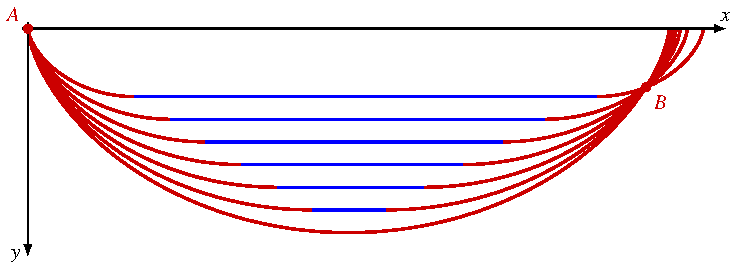
\includegraphics{chapters/020-variation/images/singulaer.pdf}
\caption{Verschiedene Lösungen unter Verwendung der singulären Lösungen
der Differentialgleichung der Brachistochronen.
Die roten Kurventeile sind Lösungen der ursprünglichen
Brachistochronengleichung
\eqref{XXX},
die blauen Teile sind durch die Multiplikation mit $y'$ in
\eqref{buch:variation:eulerlagrange:eqn:multiplikation}
hinzugekommen, sind aber nicht Lösungen der ursprünglichen
Gleichungen.
Nur die untereste Kurve ist daher eine Brachistochrone.
\label{buch:variation:eulerlagrange:fig:brachloes}}
\end{figure}

Die Differentialgleichung
\eqref{buch:variation:eulerlagrange:eqn:brachistochrone1}
hat die Lösung $y(x)=C$, denn in diesem Fall verschwindet
der Zähler und die Differentialgleichung wird zu $y'(x)=0$,
was für die Konstanten $C$ natürlich erfüllt ist.
Der Satz von Picard-Lindelöf besagt, dass die Lösung einer
Differentialgleichung $y'=f(x,y)$ eindeutig bestimmt ist, wenn die rechte
Seite eine Lipshitz-Bedingung erfüllt.
Dies ist für die rechte Seite von
\eqref{buch:variation:eulerlagrange:eqn:brachistochrone1}
nicht gegeben, die Lösung ist daher nicht eindeutig bestimmt.

Die Zykloide~\eqref{buch:variation:eulerlagrange:eqn:zykloide}
erreicht den tiefsten Punkt bei $t=\pi$, die $y$-Koordinate ist
$y(\pi)=C$.
In diesem Punkt ist die Lösungskurve horizontal.
Da die Lösung an diesem Punkt nicht eindeutig bestimmt ist,
kann sie mit der konstanten Funktion fortgesetzt werden
(Abbildung~\ref{buch:variation:eulerlagrange:fig:brachloes}).
Ebenso kann die Lösung an einer beliebigen Stelle mit dem ansteigenden
Teil der Zykloide fortgesetzt werden.

Woher kommen diese singulären Lösungen?
Eine konstante Lösung $y(x)=C$ hat Ableitungen
$y'(x)=0$ und $y''(x)=0$.
Eingesetzt in die ursprüngliche Gleichung
\eqref{buch:variation:eulerlagrange:eqn:brachistochrone0}
(Form auf der linken Seite) ergibt
\[
0
=
1+y'(x)^2+2y(x)y''(x)
=
1 + 0^2 + 2C\cdot 0
=
1.
\]
Dieser Widerspruch zeigt, dass die singulären Lösungen nicht
Lösungen der Euler-Lagrange-Differentialgleichungen sind, sondern
durch die Multiplikation mit $y'$ in
\eqref{buch:variation:eulerlagrange:eqn:multiplikation}
entstanden sind.

